\section{Construction: The Precompile Suite and PLUM-in-BDEC}\label{sec:system}

The theoretical analysis of Section~\ref{sec:theoretical} identified the algebraic-hash and large-prime-field operations of PLUM verification as the operations that carry the field-mismatch tax inside a small-field zkVM. This section presents the instrument we built to absorb that tax so that the remaining proving cost can be measured: a precompile suite, developed in two stages, and its integration into the BDEC credential-generation relation. The suite serves the measurement reported in Section~\ref{sec:evaluation}. Its purpose is to move the dominant cost out of emulated guest code so that what remains can be measured, attributed, and bounded. Throughout, we grade the evidence supporting each component, distinguishing what is proved from what is empirically tested and what is trusted from upstream, since the suite is not uniformly sound. Two soundness questions are left explicitly open (\S\ref{ssec:soundness}); a measurement whose correctness rested on unstated assumptions would be worth little, so stating the open questions is part of the work. The same Griffin chip that lowers the core-layer cost enlarges the recursion verifier's core machine, and that enlargement, quantified in Section~\ref{sec:evaluation}, is what the zero-knowledge wrap obstruction inherits.

\subsection{Scope of the Implementation}\label{ssec:impl-scope}
We state plainly what is and is not built, since the honesty of every measurement in Section~\ref{sec:evaluation} depends on this scope being explicit.

\begin{itemize}
  \item \textbf{Fp192 modular multiplication via the host precompile}
  (\S\ref{ssec:bigint}), routed through SP1's \texttt{UINT256\_MUL} and RISC~Zero's \texttt{sys\_bigint}, implemented for both targets. \emph{Built; reduction argued; empirically tested (14/14 adversarial cases).}
  \item \textbf{A bespoke Griffin-$\mathbb{F}_p^{192}$ permutation AIR for SP1} (\S\ref{ssec:griffin-air}), the load-bearing precompile, since PLUM's constraint budget is dominated by Griffin. All ten constraint families implemented ($\approx 3{,}900$ lines of Rust across the chip and executor-compute modules, over $24$ commits); a single-permutation smoke proof completes (execute$+$prove$+$verify) in $13.0$~s on the target hardware. \emph{Built; constraint-level chip-equivalence not yet verified (\S\ref{ssec:soundness}).}
  \item \textbf{PLUM signature verification on SP1}, suite active. \emph{Built; proves end-to-end} ($14.89$--$32.5$~min at $\lambda=80$, build- and machine-state-sensitive, tuned memory configuration; Section~\ref{sec:evaluation}).
  \item \textbf{PLUM signature verification on RISC~Zero} (standalone guest, Griffin hasher emulated in guest code, field arithmetic via \texttt{sys\_bigint}). \emph{Built; proves end-to-end} ($6$\,h\,$19$\,m at $\lambda=80$; Section~\ref{sec:evaluation}).
  \item \textbf{PLUM-in-BDEC credential generation (CreGen) on RISC~Zero}, with field arithmetic via \texttt{sys\_bigint}. \emph{Built; validated in execute mode} ($9.4\times10^{9}$ guest cycles, both signature verifications accepting); its succinct proof on RISC~Zero did not yield a receipt, ending in an internal-verifier rejection under diagnosis rather than a resource limit; on SP1 the same relation completes a succinct prove ($26.98$ and $31.11$~min, $n=2$; receipt verified, not zero-knowledge) (Section~\ref{sec:evaluation}).
  \item \textbf{PLUM-in-BDEC presentation (ShowCre) on RISC~Zero}, the $k+2$-verification generalisation of CreGen. \emph{Built; validated in execute mode} at $k=1$ ($1.41\times10^{10}$ guest cycles) and $k=2$ ($1.88\times10^{10}$ cycles), all $k+2$ verifications accepting; its succinct proof on RISC~Zero was not attempted, sharing CreGen's prover path, whereas on SP1 it completes a succinct prove ($40.15$ and $44.24$~min at $k=1$, $n=2$; $58.14$~min at $k=2$, $n=1$; receipt verified, not zero-knowledge) (Section~\ref{sec:evaluation}).
\end{itemize}

\noindent One component is deliberately \emph{not} built, and we treat it as future work: a port of the bespoke Griffin AIR to RISC~Zero's syscall ABI. For reading Section~\ref{sec:evaluation} this matters, because ``the precompile'' does not denote one artefact uniform across both zkVMs. On SP1 the suite includes the bespoke Griffin AIR. On RISC~Zero the same arithmetic is carried by \texttt{sys\_bigint}. We state which mechanism is active wherever a measurement is reported.

\subsection{The Field-Arithmetic Substrate: \texttt{Fp192} Multiplication via the Host Precompile}\label{ssec:bigint}
\paragraph{Field and naming.}
PLUM operates over the prime field $\mathbb{F}_p$ with $p = 2^{64}\cdot p_0 + 1$, $p_0$ a $135$-bit prime, so $p$ is a \emph{$199$-bit} prime. We retain the label ``$\mathbb{F}_p^{192}$'' for parity with the PLUM paper, whose \S3.3 titles the parameter ``$192$-bit smooth prime field''; all soundness arguments use the true $199$-bit modulus, which is fixed in the implementation and audited against the paper.\footnote{Two distinct points must not be conflated. (i) The $192$-vs-$199$ \emph{label} is a naming convention: PLUM's \S3.3 titles the field ``$192$-bit'' while the concrete modulus is $199$ bits; we keep the paper's label but compute with the true value. (ii) Separately, the specific decimal prime is a \emph{substitution}: as recorded in Remark~\ref{rem:prime-substitution} and the open prime-instantiation hypothesis of Section~\ref{sec:security}, the value used is a nearby prime satisfying PLUM's structural requirements, and any bit-exact security claim is conditional on it matching the intended parameters. This conditional dependence is an open item rather than a naming convention.}

\paragraph{Construction.}
We do not write a dedicated $199$-bit multiplication circuit. Both target zkVMs already ship a $256$-bit modular-multiplication precompile modulo a runtime-supplied modulus: SP1's \texttt{UINT256\_MUL} and RISC~Zero's \texttt{sys\_bigint(OP\_MULTIPLY)}~\cite{succinct2024sp1,bruestle2023risczero}. Each \texttt{Fp192} multiplication $a\cdot b \bmod p$ is computed by zero-padding $a$, $b$, and $p$ into the precompile's $256$-bit slots and invoking the syscall with modulus $m=p$. The wiring is selected at compile time per target.

\paragraph{Soundness (reduction).}
\begin{description}
  \item[Upstream assumption.] For every row of the host modular-multiplication table in a verifying proof, the host AIR enforces $x' \equiv x\cdot y \pmod{m}$ and $x' \in [0,m)$ when $m\neq 0$. For SP1 we point to the two specific AIR constraints that enforce these (the modular product and the output range check); for RISC~Zero the same guarantee is enforced by auto-generated constraint code that we \emph{cite} as production-audited rather than re-derive. This RISC~Zero citation is the weakest link and is graded accordingly. The precompiles are those of SP1 v6.2.1 (forked) and RISC~Zero 3.0.5 (\texttt{risc0-circuit-rv32im} 4.0.4), the versions the repository build resolves; the CreGen anomaly run of Section~\ref{sec:evaluation} ran on the same build (the compiled library embeds the 3.0.5 sources, built thirteen days before that run). The assumption is thus pinned to these specific versions and not to an unversioned ``upstream release process.''
  \item[Reduction.] \texttt{Fp192} operands are maintained in $[0,p)$ (structurally for the reducing constructor, by input domain for the small-integer constructors). Since $p < 2^{200} < 2^{256}$, the zero-pad is the identity on the bit pattern. The assumption with $m=p$ yields $x' = a\cdot b \bmod p \in [0,p)$, exactly the value the software fallback computes; the implementation reconstructs the field element directly from $x'$, omitting a redundant reduction, with a debug-build assertion guarding against regression of the upstream range check.
\end{description}

\paragraph{Edge cases.}
The argument addresses a malicious modulus $m=0$ (prevented by loading the modulus from a compile-time constant the zkVM's memory checking binds), non-canonical operand truncation (guarded by a debug assertion on operand width), and regression of the upstream range check (under which the omitted reduction would become load-bearing, detected by the same assertion).

\paragraph{Empirical corroboration.}
An adversarial probe exercises an honest control plus six single-field tamper cases (corrupted public key, message, and four signature fields: the $\sigma_1$ Merkle root, the PRF tag, a virtual-oracle response, and a final STIR coefficient) on each zkVM; all $14$ cases across both platforms behave as expected (honest accepts, every tamper rejects). This is regression evidence; it does not characterise malicious-prover behaviour completely, and we report it as such.

\subsection{The Bespoke Griffin-$\mathbb{F}_p^{192}$ Permutation AIR (SP1)}\label{ssec:griffin-air}

\begin{figure}[t]
\centering
\begin{tikzpicture}[
  >={Stealth},
  every node/.style={font=\footnotesize},
  s/.style={align=center, text width=25mm},
  node distance=7mm and 10mm,
]
  \node[s] (op) {$\mathbb{F}_p^{199}$ operation (Griffin)};
  \node[s, above right=4mm and 10mm of op] (e1) {multi-limb emulation ($\approx7$ limbs)};
  \node[s, right=of e1] (e2) {huge trace};
  \node[s, right=of e2] (e3) {\textbf{DNF / OOM} ($1$m$45$s)};
  \node[s, below right=4mm and 10mm of op] (s1) {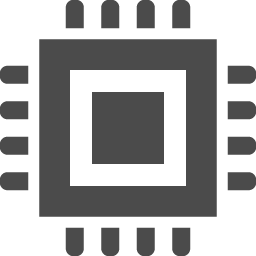
\includegraphics[height=7mm]{figs/assets/cpu.png}\\ syscall to native chip};
  \node[s, right=of s1] (s2) {cross-table lookup};
  \node[s, right=of s2] (s3) {trace $\to$ receipt (host-side cost)};
  \draw[->] (op) -- (e1); \draw[->] (e1) -- (e2); \draw[->] (e2) -- (e3);
  \draw[->] (op) -- (s1); \draw[->] (s1) -- (s2); \draw[->] (s2) -- (s3);
\end{tikzpicture}
\caption{Where the field-mismatch tax is incurred and what the precompile absorbs.
Left: each $\mathbb{F}_p^{199}$ operation expands into multi-limb arithmetic that,
un-precompiled, does not complete (OOM at $1$m$45$s). Right: a syscall routes it to a
native chip, the bespoke Griffin AIR on SP1 or \texttt{sys\_bigint} on RISC~Zero
(\emph{not} one artefact), bound to the trace by a cross-table lookup; the chip's
cost is charged host-side, so a guest-cycle saving need not be a wall-clock one.}
\label{fig:fmt-precompile}
\end{figure}
No existing SP1 chip computes a Griffin permutation over a $199$-bit prime field; the closest upstream pattern is SP1's Poseidon2 chip~\cite{succinct2024sp1}, implementing the Poseidon2 permutation~\cite{grassi2023poseidon2}, which has the same shape (a permutation precompile with single-pointer state I/O, per-round columns, and memory binding) but operates over SP1's $31$-bit base field (KoalaBear, $2^{31}-2^{24}+1$, in the evaluated fork). We therefore implement a custom AIR for one Griffin-$\pi$ permutation over $\mathbb{F}_p^{4}$, exposed to the guest as a single syscall on a $16$-word ($4$-lane) state.

\paragraph{Per-round constraints.}
Each of the $14$ rounds is encoded by five per-round constraint families (the round-function families of Appendix~\ref{app:proofs}): a degree-$3$ forward S-box on one lane; an \emph{inverse} S-box on another lane, constrained in the backward direction ($y^d = x$ with the root witnessed) because the forward inverse exponent is a $199$-bit number that would blow past the constraint-degree budget, valid because $\gcd(d,p-1)=1$ makes the cube map a bijection, so the witnessed root is unique; this side condition is \emph{not} automatic and we verify it for the implemented modulus: with $d=3$ and $p = 2^{64}p_0+1$ we have $p-1 = 2^{64}p_0\equiv p_0\equiv 1\pmod 3$ (since $2^{64}\equiv 1\pmod 3$, and $p_0\equiv 1\pmod 3$ for the implemented $199$-bit modulus, verified by computation), hence $3\nmid(p-1)$ and $\gcd(3,p-1)=1$ (were $3\mid(p-1)$ the cube would be three-to-one and a malicious prover could witness a wrong root); a quadratic layer on the remaining two lanes; the linear layer (the circulant $[2,1,1,1]$, which is invertible but not MDS, unlike Griffin's standard width-$4$ matrix); and the SHAKE256-derived round constants. The chip's remaining five families (round count, memory binding, output canonicality, row scheduling, parameter immutability) constrain the trace as a whole, as described next. The modulus, round count, linear-layer entries, round constants, and quadratic coefficients are bound in preprocessing rather than supplied per row, so a prover cannot choose them. A separate controller chip binds the syscall's memory reads and writes, and a per-lane output range check enforces output canonicality (\S\ref{ssec:bigint}'s cross-precompile contract). Two audit-driven hardening passes fixed a polynomial-degree blow-up and an all-zero-padding-row identity failure.

\paragraph{What works.}
A single-permutation smoke proof passes execute, prove, and verify in $13.0$~s on the target hardware, establishing the per-syscall proving cost in isolation.

\subsection{The Sponge and Compression Wrapper}\label{ssec:sponge}
The permutation is wrapped in the sponge/compression construction of the Loquat instantiation to provide the $2$-to-$1$ compression used by the BDEC Merkle trees. The state width is $t_{\mathsf{state}}=4$, the capacity $c_{\mathsf{cap}}=2$, and the rate $r=t_{\mathsf{state}}-c_{\mathsf{cap}}=2$, so a digest is the first two lanes of the output state. The $2$-to-$1$ compression of two child digests $x=(x_0,x_1)$ and $y=(y_0,y_1)\in\mathbb{F}_p^{2}$ is $H_2(x,y)=\big(\pi(x_0,x_1,y_0,y_1)\big)_{0,1}$: one application of the width-$4$ permutation $\pi$, truncated to the rate lanes. The SHAKE256 domain-separation seed and the linear-layer matrix are matched to the reference hasher, and cross-codebase tests pin the modulus, round count, linear-layer matrix, and seed against the reference implementation.

\subsection{Soundness of the Precompile Suite, and Two Open Questions}\label{ssec:soundness}
This subsection states the soundness claim and the two questions it leaves open. The per-constraint audit is deferred to Appendix~\ref{app:proofs}.

\begin{theorem}[Precompile soundness, conditional]\label{thm:precompile-sound}
This is a functional (input--output) equivalence statement, and, conditional on the black-box-transfer hypothesis, a transfer of PLUM's EU-CMA reduction; it is not a standalone cryptographic-security claim. Assume the host zkVM's cross-table lookup argument is sound; Assumption~\ref{asm:air} (the Griffin AIR's constraints are satisfied only by a witnessed transition equal to the reference Griffin-$\pi$ permutation); and that PLUM's EU-CMA reduction treats Griffin and field multiplication as black-box input--output maps, inspecting no intermediate representation (such as a limb of a field product); together with the upstream modular-multiplication guarantee of \S\ref{ssec:bigint}. Then substituting the precompile suite for the emulated operations preserves the input--output value of every PLUM and BDEC verification predicate. Consequently, under the black-box-transfer hypothesis, PLUM's EU-CMA reduction transfers unchanged: that reduction is in the random-oracle model and depends only on the input--output behaviour of the hash function instantiating the oracle, which, granting Assumption~\ref{asm:air}, the precompile reproduces \emph{exactly}: under that assumption it computes the same function the emulated code did, so no random-oracle programming step in the reduction is affected. (The reduction's reliance on (Q)ROM-replaceability of this Griffin instantiation is a separate, upstream assumption, recorded as an open upstream assumption in Section~\ref{sec:security} and not discharged here.)
\end{theorem}

\paragraph{What is established.}
The field-substrate half rests on the reduction of \S\ref{ssec:bigint}. The suite is platform-specific: on SP1 it includes the bespoke Griffin AIR, to which Assumption~\ref{asm:air} applies; on RISC~Zero the Griffin arithmetic is carried by \texttt{sys\_bigint} emulation, so Assumption~\ref{asm:air} is not invoked there and is replaced by the analogous input--output equality of the emulated permutation. For the Griffin AIR, the per-family analysis (Appendix~\ref{app:proofs}) exhibits, family by family, the constraint \emph{intended} to catch any deviation from reference Griffin, the forgery that deviation would enable, and the implementation status of each; memory binding, output canonicality, parameter immutability, and row scheduling are implemented and constrained. What that analysis does \emph{not} establish, and says so explicitly, is that the implemented constraint system is satisfied \emph{only} by reference-equal witnesses: this is Assumption~\ref{asm:air}, the \emph{chip--constraint equality}. It is empirically supported by the $256$-vector cross-codebase agreement and the partial fault-injection coverage discussed below (per-vector false-pass probability $\approx 2^{-199}$ for the vector suite), but the vector agreement pins the \emph{executor} against the reference, a weaker \emph{chip--executor} equality, not the \emph{constraints}; Assumption~\ref{asm:air} is not verified at the constraint level.

\paragraph{Open question 1: Assumption~\ref{asm:air} is empirically supported but unproved.}
The $256$-vector agreement establishes that the executor's native compute equals the reference permutation; it does \emph{not} by itself establish that the \emph{AIR constraints} admit only that computation (that the chip witness equals the executor). For the per-row layer (the per-row families) that stronger statement now carries a written proof: Appendix~\ref{app:proofs} bridges the limb identities the chip constrains over its small base field to congruences modulo $p$ and composes them into the reference round, conditional only on the byte-range lookups that the lookup-binding hypothesis already covers. A separate fault-injection suite corroborates this layer in the rejection direction via \texttt{debug\_constraints}: single-cell corruptions of a satisfying trace are rejected for each of the seven families. The lookup-borne families (round count, memory binding, and the cross-row threading of row scheduling) lie outside both the proof and that harness and require a full-prover harness; parameter immutability is argued by construction. What Assumption~\ref{asm:air} still carries is the fidelity of the code-to-constraint transcription together with the lookup-borne families; closing it requires deriving the AIR witness from the same reference code and checking constraint satisfaction directly, ideally by machine.

\paragraph{Open question 2: the QROM status of this Griffin instantiation is upstream of the AIR.}
PLUM's EU-CMA argument under Fiat--Shamir requires Griffin to be replaceable by a (quantum) random oracle. The Griffin analyses cover the original instantiations; whether they cover this $d=3$, width-$4$, $199$-bit-field, $14$-round instantiation is not something the AIR can settle. If this instantiation were QROM-distinguishable, no amount of AIR engineering would recover security. We flag this as a thesis-level assumption that still has to be checked against the Griffin literature; we do not close it here.

\paragraph{Further limitations not hidden.}
The RISC~Zero \texttt{sys\_bigint} soundness is cited from the upstream release process rather than re-derived; the EU-CMA reduction is argued to transfer on the grounds that the reference reduction treats Griffin and field multiplication as black-box input--output maps, but we have not audited PLUM's reduction line by line for a step that inspects an \emph{intermediate} representation (such as a limb of a field product), which input--output equality alone would not cover; and the zero-knowledge property required by BDEC's anonymity guarantee is a property of the proof wrap, analysed as the security--deployability tension of Section~\ref{sec:security} and measured in Section~\ref{sec:evaluation}, not closed here.

\subsection{Integration into the BDEC Credential-Generation Relation}\label{ssec:integration}
The credential-generation relation $R_{\mathsf{cre}}^{\mathsf{PLUM}}$ of Section~\ref{sec:prelim} is the AND concatenation of two PLUM signature verifications, both under the user's public key $\pk_U$, with public statement $x_{\mathsf{cre}}=(c_{U,TA},h_{U,TA},\mathsf{ppk}_{U,TA})$ and witness $w_{\mathsf{cre}}=(\pk_U,\mathsf{psk}_{U,TA})$. We implement this relation \emph{in full} as a RISC~Zero guest, with PLUM in place of Loquat and field multiplications routed through \texttt{sys\_bigint}; the guest computes exactly the two $\Pred_{\Verify}$ conjuncts that define base CreGen, with no omitted predicate. (The optional Merkle-accumulator variant of Remark~\ref{rem:merkle-extension} is not part of this relation and performs its membership checks in $\BDEC.\mathsf{ShowVer}$; it is out of scope here.) One \emph{statement-binding} requirement remains open at the receipt level, and it bears on security, so we do not treat it as a cosmetic completeness gap: the prototype commits the verification outcome to the journal but not yet the public statement $x_{\mathsf{cre}}$ itself, so a receipt currently attests ``two signatures verify under some witness'' without binding the proof to the specific public $(c_{U,TA},h_{U,TA},\mathsf{ppk}_{U,TA})$. Until $x_{\mathsf{cre}}$ is committed to the journal, the artifact serves as a \emph{functional benchmark} and does not yet act as a statement-bound credential verifier: an accepting receipt does not certify \emph{which} statement was proved. Committing $x_{\mathsf{cre}}$ is a small, cost-negligible change (a few field elements) and is noted as immediate next work (Section~\ref{sec:conclusion}); it does not alter the proved relation. In execute mode at $\lambda=80$ the guest runs both verifications to acceptance in $9.4\times10^{9}$ guest cycles, the two costing essentially the same ($\approx 4.69\times10^{9}$ each), confirming that both pass through the same precompile-backed path. The transition from this execute-mode validation to a completed proof is the subject of Section~\ref{sec:evaluation}. On SP1 both relations complete a succinct (non-zero-knowledge) prove: CreGen in $26.98$ and $31.11$~min, ShowCre in $40.15$ and $44.24$~min at $k=1$ and $58.14$~min at $k=2$ (Section~\ref{sec:evaluation}), a receipt distinct both from RISC~Zero's internal-verifier rejection above and from the still-open zero-knowledge wrap. The full presentation relation (ShowCre), the $k+2$-verification generalisation of this relation, is likewise implemented as a RISC~Zero guest and validated in execute mode at $k=1,2$ (Section~\ref{sec:evaluation}); its zero-knowledge proof, like CreGen's, has not been produced on the target hardware (Section~\ref{sec:evaluation}).
